
\Section{Sheaves}
\Definition{
$X$を位相空間とする.$X$上の(アーベル群の)\textbf{前層}(presheaf)$\, \mathcal{F}$とは
次のデータ
\begin{center}
  \begin{itemize}
    \item[---] $U$を任意の$X$の開集合に対して$\mathcal{F}(U)$はアーベル群.
    \item[---] 制限写像(restriction map)と言われる群準同型
          $\rho_{U,V}:\mathcal{F}(U) \to \mathcal{F}(V)$が任意の開集合$V\subset U$に対して存在する.
  \end{itemize}
\end{center}
そして次の条件を満たす.
\begin{itemize}
  \item[(1)] $\rho_{U,U} = \text{id}_{\mathcal{F}(U)}$
  \item[(2)] 任意の開集合$W\subset V \subset U$に対して$\rho_{U,W}=\rho_{V,W}\circ \rho_{U,V}$となる.
\end{itemize}
}
$s\in \mathcal{F}(U)$を$U$上の$\mathcal{F}$の\textbf{切断}(section)という.
また,$\rho_{U,V}(s)\in \mathcal{F}(V)$を$s|_{V}$と書いて$s$の$V$への制限という.\\
また,単に$\mathcal{F,G,H,}\dots$などと書いたら(前)層を表すことや、$\rho$と書いたら制限写像を意味する。
また,どの(前)層の制限写像かを明示するため,例えば,$\rho_{U,V}^{\mathcal{F}}$などと書くことがある。
\Definition{
前層$\mathcal{F}$が層(sheaf)とは次の条件を満たすことをいう.
\begin{itemize}
  \item[(4)] (Uniqueness) $U$を$X$の開集合とし$\{U_{i}\}_{i}$をその開被覆とする.
        $s\in \mathcal{F}(U)$が任意の$i$に対して$s|_{U_{i}}=0$ならば$s=0$
  \item[(5)] (Glueing local sections) 上の状況で,$s_i \in \mathcal{F}(U_i)$が
        $s_{i}|_{U_{i} \cap U_{j}} = s_{j}|_{U_{i} \cap U_{j}}$を満たすならば,$s|_{U_{i}} = s_{i}$を満たす$s\in \mathcal{F}(U)$が存在する.
\end{itemize}
}
\Remark{
$\mathcal{F}$が層ならば$\mathcal{F}(\varnothing) = 0$となる.
}{}
\Example{
$X$を位相空間とする.\\
$\mathcal{C}_{X}^{0}$を$X$の開集合$U$に対して$U\to \mathbf{C}$なる連続写像全体の集合$\mathcal{C}_{X}^{0}(U)$を対応させるものとし,制限写像を普通の制限とする.
\begin{equation*}
  \mathcal{C}_{X}^{0}(U) = \left\{ f:U \to \mathbf{C} \mid f\text{ is continuous} \right\}
\end{equation*}
すると,$\mathcal{C}_{X}^{0}$は$X$上の層となる.
}{
$V \subset U$なる開集合$U,V$に対して$U$上の連続写像$f\in \mathcal{C}_{X}^{0}(U)$を$V$に制限することによって得られる
$V$上の連続写像を$\rho_{U,V}(f)(=f|_{V})$と書く.すると,これは$\mathbf{C}$上のベクトル空間($\mathbf{C}$上の関数空間)
の準同型$\rho_{U,V}:\mathcal{C}_{X}^{0}(U) \to \mathcal{C}_{X}^{0}(V)$となる.つまり$(\mathcal{C}_{X}^{0},\rho)$は前層となる.\\
また,(4)を満たすのは明らかで.(5)もすぐに成り立つことがわかる.$\{U_{i}\}_{i}$を$U$の開被覆とする.$f_{i} \in \mathcal{C}_{X}^{0}(U_{i})$が
$f_{i}|_{U_{i} \cap U_{j}} = f_{j}|_{U_{i} \cap U_{j}}$を満たすとする.するとそれらを張り合わせた関数を$f$とすればこれは
$f\in \mathcal{C}_{X}^{0}(U)$であり,$f|_{U_{i}}=f_{i}$となる.よって$(\mathcal{C}_{X}^{0},\rho)$は層となる.これを連続写像が成す層という.
}
\Example{
$X$を位相空間とする.\\
$A$を自明でないアーベル群とする.$\mathcal{A}_{X}$を$X$の空でない開集合$U$に対して$\mathcal{A}_{X}(U)=A$に,
空集合$\varnothing$に対して$\mathcal{A}_{X}(\varnothing) = 0$に対応させるものとし,
制限写像を空でない開集合$V \subset U$に対して$\rho_{U,V}=\text{id}_{A}$とし,$\rho_{U,\varnothing} = 0$とする.\\
すると,$(\mathcal{A}_{X},\rho)$は$X$上の前層にはなるが,一般に層とはならない.\\
}{
例えば,$X$が連結でないとすると,非交差な開集合$U,V$があって$X=U\cup V$とかける.すると$\{U,V\}$は$X$の開被覆となる.
$s_{U} \in \mathcal{A}_{X}(U)=A$が$s_{U}|_{U\cap V} = s_{U}|_{\varnothing} = 0 = s_{V}|_{U \cap V}$
を満たすとする.このとき,任意の$s \in \mathcal{A}_{X}(X)=A$で$s|_{U}=s|_{V}=s$となり層とならない.
}

\Example{
(skyscraper sheaf)\\
$X$を位相空間、$A$をアーベル群とする。$p\in X$に対して$i_{p} : \{p\} \hookrightarrow X$を包含写像とする。
このとき$i_{p,*}\mathcal{A}$を
\begin{equation*}
  i_{p,*}\mathcal{A}(U) = \left\{
  \begin{alignedat}{2}
      & A \qquad & p \in U    \\
      & 1 \qquad & p \notin U
  \end{alignedat}
  \right.
\end{equation*}
と定義する。これは層になる。
}{}




\Definition{
  位相空間$X$上の前層$\mathcal{F}$と$x\in X$に対して,$x$での$\mathcal{F}$の\textbf{茎(stalk)}$\mathcal{F}_{x}$という群が定義できる.
  \begin{equation*}
    \mathcal{F}_{x} = \varinjlim_{U \ni x}\mathcal{F}(U)
  \end{equation*}
  ただし,$U$は$x$の開近傍をすべてを回る.$U$上の切断$s\in \mathcal{F}(U)$に対して
  $x\in U$の茎$\mathcal{F}_{x}$への自然な群準同型の像を$s_{x}$と書いて,$x$での$s$の\textbf{芽(germ)}という.
}

\Proposition{
  層の定義の(4),(5)を次の列が完全系列であるとすることができる.
  \begin{equation*}
    C^{\bullet}(\mathcal{U},\mathcal{F}) : 0 \longrightarrow \mathcal{F}(U) \stackrel{d_{0}}{\longrightarrow} \prod_{i}\mathcal{F}(U_{i}) \stackrel{d_{1}}{\longrightarrow} \prod_{i}\mathcal{F}(U_{i}\cap U_{j})
  \end{equation*}
  ただし,$\mathcal{U}$は開集合$U$の開被覆で$\mathcal{U} = \{U_{i}\}_{i}$.\\
  $d_{0} : s\mapsto (s|_{U_{i}})_{i},d_{1}: (s_{i})_{i} \mapsto (s_{i}|_{U_{i}\cap U_{j}} - s_{j}|_{U_{i}\cap U_{j}})_{i,j}$
}{
}

\Lemma{
$\mathcal{F}$を$X$上の層とする.$s,t \in \mathcal{F}(X)$が任意の$x \in X$に対して$s_{x} = t_{x}$ならば$s=t$
}{
差を考えれば$t=0$のときを考えればいい.$s_{x}=0\ (\forall x\in X)$とすると,$x$の開近傍$U_{x}$があって$s|_{U_{x}}=0$となる.$\{U_{x}\}_{x\in U_{x}}$は$X$の開被覆なので,$s=0$となる.
}
\Definition{
$X$上の2つの前層$\mathcal{F,G}$とする.\textbf{前層の射}$\alpha:\mathcal{F} \to \mathcal{G}$
とは,$X$の開集合$U$に対して群準同型$\alpha(U):\mathcal{F}(U) \to \mathcal{G}(U)$があって,
任意の開集合の組$V\subset U$に対して$\alpha(V)\circ \rho_{U,V}^{\mathcal{F}} = \rho_{U,V}^{\mathcal{G}}\circ \alpha(U)$を満たすことをいう.\\
$X$の任意の開集合$U$に対して$\alpha(U)$が単射ならば$\alpha$は単射であるという.(全射はうまくいかんっぽい?)
}

$\alpha:\mathcal{F} \to \mathcal{G}$を$X$上の前層の射とする.任意の$x \in X$に対して
$\alpha$から自然に誘導される群準同型$\alpha_{x}:\mathcal{F}_{x} \to \mathcal{G}_{x}$で
$(\alpha(U)(s))_{x} = \alpha_{x}(s_{x})$が$X$の任意の開集合$U,s\in \mathcal{F}(U),x\in U$で
成り立つものが取れる.\\
$\alpha_{x}$が任意の$x\in X$で全射なら$\alpha$が全射であるという.

\Example{
  $X=\mathbf{C} \mysetminus \{0\}$とし$\mathcal{F}$を$X$上の正則関数がなす層とし,
  $\mathcal{G}$を$X$上の双正則関数のなす層とする.今,任意の開集合$U$と任意の$f\in \mathcal{F}(U)$に対して$\alpha(U)(f) = \exp(f)$で定義される層の射$\alpha:\mathcal{F} \to \mathcal{G}$
  が全射であることはよく知られている.しかし$\alpha(X):\mathcal{F}(X) \to \mathcal{G}(X)$は
  全射ではない.例えば恒等写像は$\exp(f)$と書けない.
}{}
\Proposition{
  $\alpha:\mathcal{F} \to \mathcal{G}$を$X$上の層の射とする.
  \begin{center}
    $\alpha$が同型$\Leftrightarrow$ $\alpha_{x}$が同型$(\forall x \in X)$
  \end{center}
}{}
\Theorem{
位相空間$X$上の前層$\mathcal{F}$に対して,前層$\mathcal{F}$の層化(sheafification)$\mathcal{F}^{\dagger}$は存在する.
}{
$X$の開集合$U$に対して
\begin{equation*}
  \mathcal{F}^{\dagger}(U) = \left\{\sigma: U \to \prod_{x\in U} \mathcal{F}_{x}\, \middle|\,
  \begin{aligned}
    \forall x\in U,x\in \exists V\subset U:\text{open},\exists s \in \mathcal{F}(V)\, \text{s.t.}\, \sigma(y) = s_{y}\, (\forall y \in V)
  \end{aligned}
  \right\}
\end{equation*}
とする.ただし,$\sigma$は任意の$x\in U$に対して$\sigma(x) \in \mathcal{F}_{x}$とする.
また,$V \subset U$なる開集合に対し,
$$
  \begin{array}{rccc}
    \rho_{U,V}^{\mathcal{F}^{\dagger}}: & \mathcal{F}^{\dagger}(U) & \longrightarrow & \mathcal{F}^{\dagger}(V) \\
                                        & \rotatebox{90}{$\in$}    &                 & \rotatebox{90}{$\in$}    \\
                                        & \sigma                   & \longmapsto     & \sigma|_{V}
  \end{array}
$$
が定義できる.実際,任意の$x\in V$をとる.$V \subset U$であり,
$\sigma \in \mathcal{F}^{\dagger}(U)$より
\begin{center}
  $x\in \exists U_{0} \subset U$:open,$\exists s \in \mathcal{F}(U_{0})$\, s.t.\, $\sigma(y)=s_{y}\, (\forall y\in U_{0})$
\end{center}
$V_{0} = U_{0} \cap V,\quad t = s|_{V_{0}}$とすると任意の$y\in V_{0}$に対して
\begin{equation*}
  \sigma(y)=\sigma|_{V}(y)=s_{y}
\end{equation*}
さらに帰納極限の定義から
\begin{equation*}
  \sigma|_{V}(y)=t_{y}
\end{equation*}
次に$\mathcal{F}^{\dagger}(U)$がアーベル群,つまり
$\sigma,\tau \in \mathcal{F}^{\dagger}(U)$ならば$\sigma+\tau \in \mathcal{F}^{\dagger}(U)$
を示そう.\\
$\sigma,\tau \in \mathcal{F}^{\dagger}(U)$より任意の$x\in U$に対して
\begin{align*}
    & x\in \exists U_{0} \subset U:\mathrm{open},\exists s \in \mathcal{F}(U_{0})\ \mathrm{s.t.}\
  \sigma(y) = s_{y}\ (\forall y \in U_{0})                                                       \\
    & x\in \exists V_{0} \subset U:\mathrm{open},\exists t \in \mathcal{F}(V_{0})\ \mathrm{s.t.}\
  \tau(z) = t_{z}\ (\forall z \in V_{0})
\end{align*}
を満たす.いま$W = U_{0} \cap V_{0},s' = s|_{W},t' = t|_{W}$とすると,
\begin{align*}
  x\in W \subset U:\mathrm{open}, s',t' \in \mathcal{F}(W)\ \mathrm{s.t.}\
  (\sigma + \tau)(y)
    & = \sigma(y) + \tau(y)             \\
    & = s_{y} + t_{y}                   \\
    & = (s + t)_{y} \ (\forall y \in W)
\end{align*}
よって$\sigma + \tau \in \mathcal{F}^{\dagger}(U)$また明らかに可換.
よって$\mathcal{F}^{\dagger}(U)$はアーベル群.\\
また,通常の制限で制限写像を定義しているため,$\mathcal{F}^{\dagger}$は前層となる.\\
更に層となることを示そう.\\
$U$を$X$の開集合とし,$\{U_{i}\}_{i}$をその開被覆とする.$\sigma\in \mathcal{F}^{\dagger}(U)$が
任意の$i$に対して$\sigma|_{U_{i}} = 0$とする.つまり任意の$x \in U_{i}$に対して$\sigma(x) = 0$
とする.$U_{i}$は$U$を被覆するので結局$\sigma = 0$となる.\\
次に,$\sigma_{i} \in \mathcal{F}^{\dagger}(U_{i})$とし,
$\sigma_{i}|_{U_{i} \cap U_{j}} = \sigma_{j}|_{U_{i} \cap U_{j}}$と仮定すると,
$$
  \begin{array}{rccc}
    \sigma : & U                     & \longrightarrow & \displaystyle \prod_{x\in U}\mathcal{F}_{x} \\
              & \rotatebox{90}{$\in$} &                 & \rotatebox{90}{$\in$}                       \\
              & x                     & \longmapsto     & \sigma_{i}(x)
  \end{array}
$$
ただし,$x\in U_{i}$.すると,$\sigma$は$\sigma_{i}\in \mathcal{F}^{\dagger}(U_{i})$を張り合わせて作っているので
これは$\sigma \in \mathcal{F}(U)$となることが容易にわかる。よって、$\mathcal{F}^{\dagger}$は層になる。
}



\Proposition{
  層化の射$\theta:\mathcal{F} \to \mathcal{F}^{\dagger}$に対して、
  その茎の射$\theta_{x}:\mathcal{F}_{x} \to \mathcal{F}^{\dagger}_{x}$は同型である。
}{}



\Lemma{
  $\mathcal{F}$を$X$上の層とし、$\mathcal{F}'$を$\mathcal{F}$の部分層とする。
  このとき開集合$U$を$\mathcal{F}(U)/\mathcal{F}'(U)$に対応させるものは前層になる。
}{
  この対応を$\mathcal{G}$とおく。$V \subset U$なる開集合$U,V$をとる。制限写像を
  $$
    \begin{array}{rccc}
      \rho_{U,V}^{\mathcal{G}} : & \mathcal{F}(U)/\mathcal{F}'(U) & \longrightarrow & \mathcal{F}(V)/\mathcal{F}'(V)                \\
                                  & \rotatebox{90}{$\in$}          &                 & \rotatebox{90}{$\in$}                         \\
                                  & s + \mathcal{F}'(U)            & \longmapsto     & \rho_{U,V}^{\mathcal{F}}(s) + \mathcal{F}'(V)
    \end{array}
  $$
  とすると、これはwell-definedである。また、$U\subset V \subset W$なる開集合の組に対して
  \begin{equation*}
    \rho_{U,W}^{\mathcal{G}} = \rho_{V,W}^{\mathcal{G}} \circ \rho_{U,V}^{\mathcal{G}}
  \end{equation*}
  が成り立つことは制限写像の定義から明らかである。よって$\mathcal{G}$は前層。
}
\Definition{
  Lem:\ref{Lem:1.3.8}で定義した前層の層化を$\mathcal{F}/\mathcal{F}'$と書いて、\textbf{商層(quotient shaef)}という。
}
\Definition{
  $\alpha:\mathcal{F} \to \mathcal{G}$を前層の射とする。このとき開集合$U$に対して
  $U \mapsto \ker (\alpha(U))$とするものは$\mathcal{F}$の部分層になる。これを$\ker{\alpha}$と
  書いて、\textbf{$\alpha$の核(kernel of $\alpha$)}という。\\
  更に、$U\mapsto \im (\alpha(U))$は一般には前層となるので、これの層化を$\im \alpha$と書いて、
  \textbf{$\alpha$の像(image of $\alpha$)}という。\\
  また,$U\mapsto \coker (\alpha(U)) = \mathcal{G}(U)/\im (\alpha(U))$は一般には前層となるので,これの層化を$\coker \alpha$と書いて,\textbf{$\alpha$の余核(cokernel of $\alpha$)}という.
}
\Lemma{
$\mathcal{F,G}$を$X$上の層,$\mathcal{F}'$を$\mathcal{F}$の部分層,$\alpha:\mathcal{F} \to \mathcal{G}$を前層の射とする。
このとき、
\begin{align*}
    & (\ker \alpha)_{x} = \ker \alpha_{x}                               \\
    & (\im \alpha)_{x} = \im \alpha_{x}                                 \\
    & (\coker \alpha)_{x} = \coker \alpha_{x}                           \\
    & (\mathcal{F}/\mathcal{F}')_{x} = \mathcal{F}_{x}/\mathcal{F}'_{x}
\end{align*}
が成り立つ。
}{
$\mathcal{Q}(U) = \mathcal{F}(U)/\mathcal{F}'(U)$とおく。\\
このとき、アーベル群の完全列
\begin{center}
  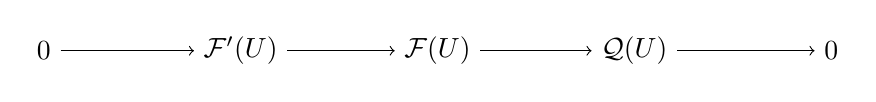
\begin{tikzpicture}[auto]
    \node (03) at (0,-1) {$0$};
    \node (im1) at (2.5,-1) {$\mathcal{F}'(U)$};
    \node (gu) at (5,-1) {$\mathcal{F}(U)$};
    \node (qu) at (7.5,-1) {$\mathcal{Q}(U)$};
    \node (04) at (10,-1) {$0$};

    \draw[->] (03) to (im1);
    \draw[->] (im1) to (gu);
    \draw[->] (gu) to (qu);
    \draw[->] (qu) to (04);
  \end{tikzpicture}
\end{center}
が作れる。帰納極限は完全列を完全列に移すので、またProp:\ref{Prop:1.3.7}より
\begin{center}
  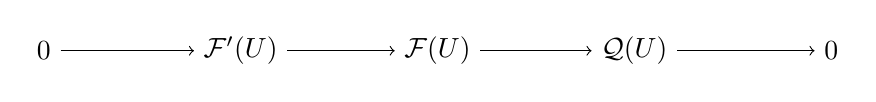
\begin{tikzpicture}[auto]
    \node (03) at (0,-1) {$0$};
    \node (im1) at (2.5,-1) {$\varinjlim \mathcal{F}'(U)$};
    \node (gu) at (5,-1) {$\varinjlim \mathcal{F}(U)$};
    \node (qu) at (7.5,-1) {$\varinjlim \mathcal{Q}(U)$};
    \node (04) at (10,-1) {$0$};

    \draw[->] (03) to (im1);
    \draw[->] (im1) to (gu);
    \draw[->] (gu) to (qu);
    \draw[->] (qu) to (04);
  \end{tikzpicture}
\end{center}
を得る。よって
\begin{center}
  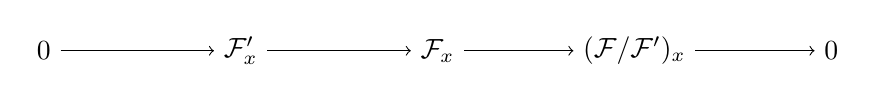
\begin{tikzpicture}[auto]
    \node (03) at (0,-1) {$0$};
    \node (im1) at (2.5,-1) {$\mathcal{F}'_{x}$};
    \node (gu) at (5,-1) {$\mathcal{F}_{x}$};
    \node (qu) at (7.5,-1) {$(\mathcal{F}/\mathcal{F}')_{x}$};
    \node (04) at (10,-1) {$0$};

    \draw[->] (03) to (im1);
    \draw[->] (im1) to (gu);
    \draw[->] (gu) to (qu);
    \draw[->] (qu) to (04);
  \end{tikzpicture}
\end{center}
したがって、
\begin{equation*}
  \mathcal{F}_{x}/\mathcal{F}'_{x} \simeq (\mathcal{F}/\mathcal{F}')_{x}
\end{equation*}
を得る。\\
次に
\begin{align*}
  (\ker \alpha)_{x}
    & = \{s_{x} \in \mathcal{F}_{x} \ |\ \alpha(U)(s) = 0,x\in U:\text{open},s\in \mathcal{F}(U) \}   \\
    & = \{s_{x} \in \mathcal{F}_{x} \ |\ \alpha_{x}(s_{x})=0,x\in U:\text{open},s\in \mathcal{F}(U)\} \\
    & = \ker \alpha_{x}
\end{align*}
を得る。同様に
\begin{align*}
  (\im \alpha)_{x}
    & = \{t_{x} \in \mathcal{G}_{x} \ |\ x\in \exists U:\text{open}, \exists s\in \mathcal{F}(U)\ \text{s.t}\ t = \alpha(U)(s)\} \\
    & = \{(\alpha(U)(s))_{x} \in \mathcal{G}_{x} \ |\ x \in U:\text{open},s\in \mathcal{F}(U)\}                                  \\
    & = \{\alpha_{x}(s_{x}) \in \mathcal{G}_{x}\ |\ s_{x} \in \mathcal{F}_{x}\}                                                  \\
    & = \im \alpha_{x}
\end{align*}
を得る.また,$(\mathcal{F}/\mathcal{F}')_{x} = \mathcal{F}_{x}/\mathcal{F}'_{x}$より
\begin{equation*}
  (\coker \alpha)_{x} = (\mathcal{G}/\im \alpha)_{x} = \mathcal{G}_{x}/\im \alpha_{x} = \coker \alpha_{x}
\end{equation*}
}

\Definition{
  層の列
  \begin{equation*}
    \mathcal{F} \stackrel{\alpha}{\longrightarrow} \mathcal{G} \stackrel{\beta}{\longrightarrow} \mathcal{H}
  \end{equation*}
  が完全とは、$\im \alpha = \ker \beta$が成り立つことをいう。
}
\Proposition{
  層の列に対して次が成り立つ。
  \begin{equation*}
    \mathcal{F} \longrightarrow \mathcal{G} \longrightarrow \mathcal{H}が完全
    \Longleftrightarrow
    任意のx \in Xに対して\mathcal{F}_{x} \longrightarrow \mathcal{G}_{x} \longrightarrow \mathcal{H}_{x}が完全
  \end{equation*}
}{
  明らか。
}

\Definition{
  $X,Y$を位相空間,$f:X\to Y$を連続写像とする。このとき、
  $X$上の層$\mathcal{F}$,$Y$上の層$\mathcal{G}$に対して、新たな$Y$上の層$f_{*}\mathcal{F}$が
  \begin{equation*}
    V \mapsto \mathcal{F}(f^{-1}(V))
  \end{equation*}
  によって定義できる。これを\textbf{$\mathcal{F}$の順像(direct image of $\mathcal{F}$)}という。\\
  また、
  \begin{equation*}
    U \mapsto \varinjlim_{V\supset f(U)}\mathcal{G}(V)
  \end{equation*}
  で定義できる新たな$X$上の前層$f^{\cdot}\mathcal{G}$の層化$f^{*}\mathcal{G}$を\textbf{$\mathcal{G}$の逆像(inverse image of $\mathcal{G}$)}
  という。
}

\Proposition{
  上の状況で
  \begin{equation*}
    (f^{*}\mathcal{G})_{x} = \mathcal{G}_{f(x)} \qquad \forall x \in X
  \end{equation*}
}{
  \begin{equation*}
    (f^{*}\mathcal{G})_{x} = \varinjlim_{x \in U}(f^{*}\mathcal{G})(U) = \varinjlim_{x \in U}\varinjlim_{f(U) \subset V}\mathcal{G}(V) = \mathcal{G}_{f(x)}
  \end{equation*}
  最後の等号は明らか.
}

\Remark{
  $V$を$Y$の開集合とする。このとき自然な単射$i:V \to Y$に対して
  \begin{equation*}
    i^{*}\mathcal{G} = \mathcal{G}|_{V}
  \end{equation*}
  が成り立つ。
}{}
\Proposition{
$f:X \to Y$を位相空間の間の連続写像とし,$\mathcal{F}$を$X$上の層.$\mathcal{G}$を$Y$上の層とする.このとき
\begin{equation*}
  \hom{\text{Sh}(X)}{f^{*}\mathcal{G}}{\mathcal{F}}\simeq \hom{\text{Sh}(Y)}{\mathcal{G}}{f_{*}\mathcal{F}}
\end{equation*}
ただし,$\hom{\mathcal{C}}{X}{Y}$は圏$\mathcal{C}$で$X \to Y$なる射全体を表し,$\text{Sh}(X)$は$X$上の層全体を表す.
}{
層化の普遍性より$\theta:f^{\cdot}\mathcal{G} \to f^{*}\mathcal{G} = (f^{\cdot}\mathcal{G})^{\dagger}$
を層化の射とすると,
$$
  \begin{array}{rccc}
      & \hom{\text{PreSh}(X)}{f^{\cdot}\mathcal{G}}{\mathcal{F}} & \stackrel{\simeq}{\longrightarrow} & \displaystyle \hom{\text{Ph(X)}}{f^{*}\mathcal{G}}{\mathcal{F}} \\
      & \rotatebox{90}{$\in$}                                    &                                    & \rotatebox{90}{$\in$}                                           \\
      & \alpha                                                   & \longmapsto                        & \tilde{\alpha}\circ \theta
  \end{array}
$$
が成り立つ.つまり
\begin{equation*}
  \hom{\text{PreSh}(X)}{f^{\cdot}\mathcal{G}}{\mathcal{F}}\simeq \hom{\text{Sh(Y)}}{\mathcal{G}}{f_{*}\mathcal{F}}
\end{equation*}
を示せばいい.次に$X$上の開集合$U$に対して
\begin{equation*}
  f^{\cdot}\mathcal{G}(U) = \varinjlim_{V\supset f(U)}\mathcal{G}(V)
\end{equation*}
なので,$\varphi \in \hom{\text{PreSh}(X)}{f^{\cdot}\mathcal{G}}{\mathcal{F}}$に対して
\begin{equation*}
  \varphi(U) : \varinjlim_{V\supset f(U)}\mathcal{G}(V) \to \mathcal{F}(U)
\end{equation*}
を与えることは帰納極限の定義より$f(U)\subset V$なる開集合$V$に対して
\begin{equation*}
  \psi'(V) : \mathcal{G}(V) \to \mathcal{F}(U)
\end{equation*}
を$f(U)\subset V' \subset V$ならば,
\begin{equation*}
  \psi'(V) = \psi'(V')\circ \rho^{\mathcal{G}}_{V,V'}
\end{equation*}
となるように与えることである.すなわち$\psi'(V)$は
\begin{equation*}
  \psi(V):\mathcal{G}(V) \to \mathcal{F}(f^{-1}(V))
\end{equation*}
と$\rho^{\mathcal{F}}_{f^{-1}(V),U}$を合成したものである.(帰納系の選び方によらない.)\\
したがって,$\varphi\in \hom{\text{PreSh}(X)}{f^{\cdot}\mathcal{G}}{\mathcal{F}}$を与えることは,$\psi \in \hom{\text{Ph}(Y)}{\mathcal{G}}{f_{*}\mathcal{F}}$を与えることと等しい.
}